
\tableofcontents
%\listoffigures
%\listoftables

% Occasionally you may find that another package defines \cleardoublepage when it
% is not required. This may cause an unwanted blank page to appear before each
% glossary. This can be fixed by redefining \glsclearpage:
% http://theoval.cmp.uea.ac.uk/~nlct/latex/packages/glossaries/glossaries-manual.html
\renewcommand*{\glsclearpage}{\clearpage}

%%%%%%%%%%%%%%%%%%%%%%%
% print the glossary  %
%%%%%%%%%%%%%%%%%%%%%%%
%\printglossary[title= Definitions,
%               toctitle=Definitions,
%               style=list,
%               ]

%%%%%%%%%%%%%%%%%%%%%%%
% print the acronyms  %
%%%%%%%%%%%%%%%%%%%%%%%
%\printglossary[type=\acronymtype,
%               title=Acronyms,
%               toctitle=Acronyms,
%               style=list
%               ]


% %%%%%%%%%%%%%%%%%%%%%%%n
% % print the symbols  %
% %%%%%%%%%%%%%%%%%%%%%%%
% \printglossary[type=symbols,
%                title=Symbols,
%                toctitle=Symbols,
%                style=list
%                ]
 
%%%%%%%%%%%%%%%%%%%%%%%%%%%%%%%%%%%%%%%%%%%%%%%%%%%%%%%%%%%%%%%%%%%%%
%% WORK STARTS HERE ......................................
%%%%%%%%%%%%%%%%%%%%%%%%%%%%%%%%%%%%%%%%%%%%%%%%%%%%%%%%%%%%%%%%%%%%%

\chapter{Rezumatul proiectului}

Proiectul 4.5G își propune implementarea unei punți între tehnologiile
curente 4G și cele emergente 5G. Această punte se realizează la
nivelul transport (TCP) prin folosirea noului protocol de transport
MPTCP pentru a utiliza în mod transparent, cumulativ si simultan
tehnologiile de rețea existente, în principal 3G/4G și WiFi, dar
potențial și alte tehnologii de comunicatie disponibile pe mobile în
viitor.


Scopul proiectului este de a instrumenta terminale Android existente,
astfel încât upgrade-ul la MPTCP nu aduce un regres de uzabilitate sau
necesitatea recompilării aplicațiilor. Avantajele aduse sunt {\bf
  conectivitatea continuă} la schimbarea rețelei WiFi sau 4G, {\bf
  capacitatea crescută} când ambele rețele sunt prezente, și {\bf
  viteză ridicată de răspuns} pentru aplicațiile interactive.


\section{ Nivel de maturitate al tehnologiilor (Tehnology Readiness Levels)}

Proiectul a demarat la nivelul TRL2, avănd beneficii clare pentru
operatori și utilizatori finali, si o literatură de specialitate care
include experimente incipiente, implementări propuse, și unele măsurători. 

Pe parcursul proiectului, mai multe etape specifice TRL3 au fost
atinse - mai multe arhitecturi de proxy au fost evaluate analitic si
experimental, arhitectura aleasă implicând folosirea RTT (round trip
time) care afectează utilizatorii.  

Livrabilul final al proiectului este un demonstrator situat la nivelul
TRL4: un telefon instrumentat și serverul proxy asociat de plasat la
operatorul 4G au fost testate într-un mnediu controlat dar realistic
la partenerul Orange Romania. Componentele au fost validate prin teste
în rețeaua 4G și WiFi, și prototipul este valid ca funcționalitate și
performanță.

\pagebreak

\section{Imagini reprezentative}

\begin{figure}[h]
	\centering
	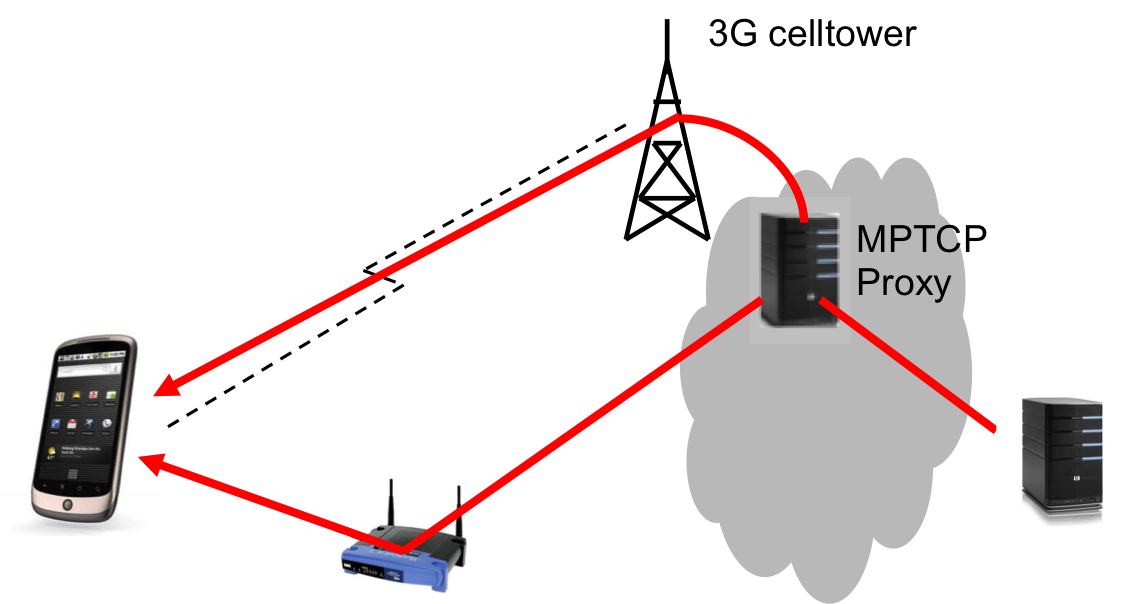
\includegraphics[scale=0.7]{figures/45g_proxy.png}
	\caption{Comunicația prin proxy}
\end{figure}


%% \begin{figure}[h]
%% 	\centering
%% 	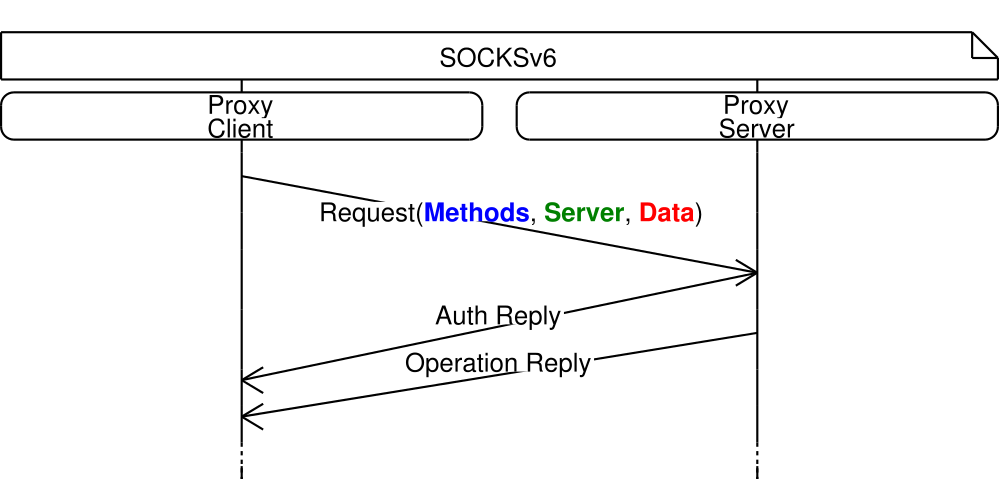
\includegraphics[scale=0.7]{figures/socks/socks6op2nd.png}
%% 	\caption{Mod de operare SOCKS 6 (conexiuni ulterioare)}
%% \end{figure}

\begin{figure}[h]
        \centering
        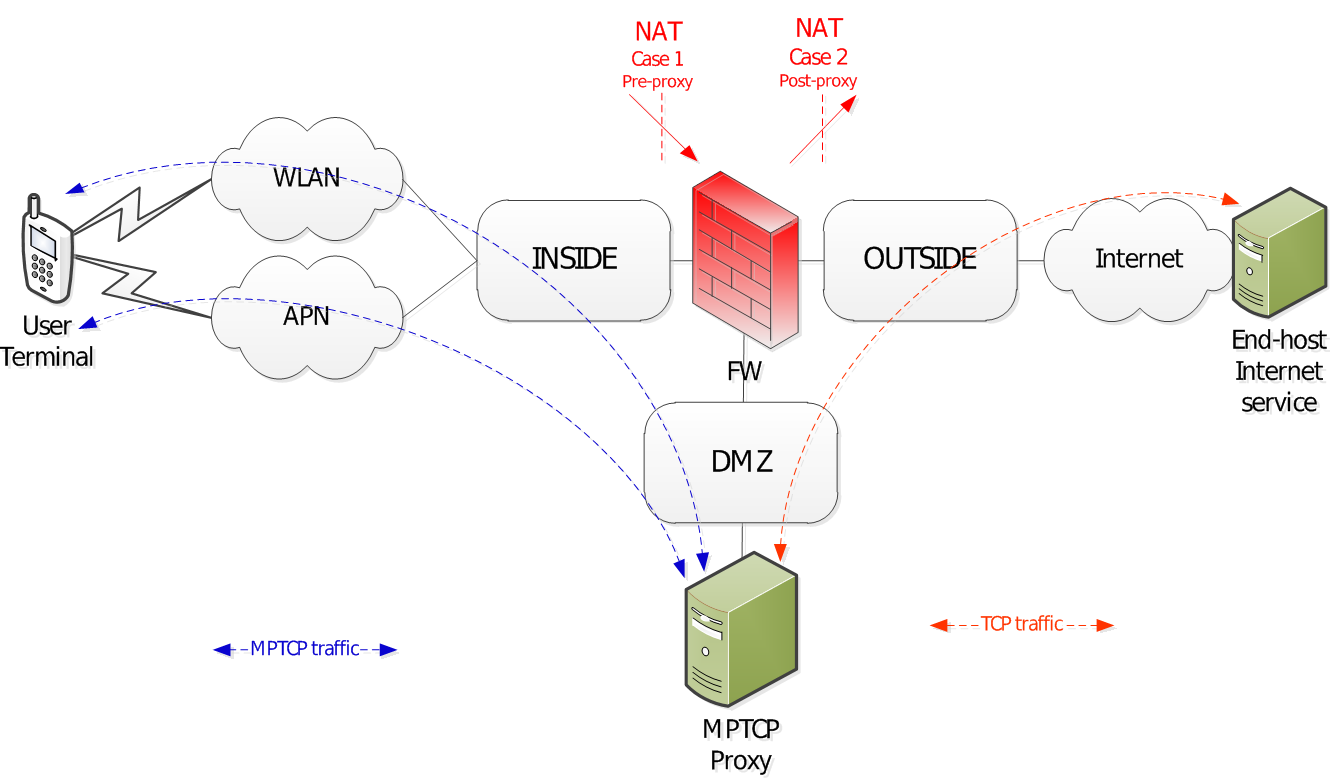
\includegraphics[scale=0.3]{figures/oro/oro_mptcp.png}
        \caption{Plasarea proxy-ului de MPTCP în rețeaua Orange Romania}
\end{figure}


 

\chapter{Obiective}
\label{sec:objectives}



\begin{itemize}
\item Implementarea modificărilor necesare pe telefoane: modificarea
kernel-ului și actualizări la Android pentru a folosi
MPTCP. Sistemul Android se bazează pe Linux, dar există suficiente
diferențe și părți specifice dispozitivului pentru a face un port
compatibil cu toate aplicațiile non-trivial.

\item Implementare și plasare proxy în rețeua Orange România
SGiLAN. Proxy-ul poate fi explicit sau transparent, fiecare soluție necesită
o implementare diferită pe telefon și la proxy.


\item Executare măsurători de performanță pentru diferite scenarii
  pentru a optimiza: conectivitatea, capacitatea, experiența cât mai
  fluidă a utilizatorului. Deoarece actualizarea MPTCP este invazivă
  pentru stiva TCP/IP, nu trebuie să existe nicio regresie a
  funcționalității sau performanțelor atunci când serviciul este
  implementat într-o rețea de testare cu o utilizatori reali.


\item Realizarea unui prototip pentru testarea la scară mai largă,
  folosind echipe de testare ale operatorului sau grupuri de
  utilizatori specializați.


\end{itemize}

\chapter{Arhitecturi de conectare  MPTCP prin proxy}
\label{sec:arch_upb}

MPTCP RFC\cite{rfc6824bis}, How hard can it be \cite{mptcp-nsdi}

\section{Background}
\section{SOCKS}


\chapter{Folosirea MPTCP în sistemul de operare Android}
\label{sec:mptcp_android}
\section{Imaginea Android}

În acest proiect s-au folosit dispozitive mobile Samsung Galaxy S7 Edge. Acestea rulează în mod implicit o imagine a sistemului de operare Android de la Samsung, care include implementarea protocolului MPTCP în kernel. 

Imaginea de Android (stock ROM) folosită este identificată prin urmatoarele:
\begin{enumerate}
	\item Model number: SM-G935F
	\item Baseband version: G935FXXU1DQA3
	\item Build number: NRD90M.G935FXXU1DQAS
	\item Android version: 7.0
\end{enumerate}

Imaginea de Android stock este rescrisă folosind utilitarul Odin, în timp ce dispozitivul este în modul \texttt{Download}. Astfel, se vor rescrie partițiile boot, system și recovery ale dispozitivului. Prin această metodă, telefonul este adus înapoi la starea inițială, în cazul întâlnirii unei erori pe parcursul root-ării dispozitivului. 

\section{Rootarea dispozitivului mobil}

Pentru activarea și configurarea protocolului MPTCP este nevoie de un telefon rootat deoarece comenzile necesare nu pot fi rulate decat din contul root (sysctl, ip rule, ip route).

Pentru root-area dispozitivului este nevoie de utilitarele Odin, TWRP și SuperSU. Se foloseste imaginea de recovery TWRP pentru modelul \emph{hero2lte}. Se scrie această imagine folosind Odin, în timp ce telefonul este în modul \texttt{Download}. Astfel, se va rescrie partiția de recovery a dispozitivului. 

Apoi se intră în modul \texttt{Recovery} al telefonului pentru a accesa meniul aplicației TWRP. Se formatează partiția de date și se instalează aplicația SuperSU care rootează telefonul. 

În final se boot-ează telefonul în modul normal si se instalează aplicația Android TWRP. Apoi, în adb shell se poate introduce comanda \texttt{su} pentru a intra în contul utilizatorului root. Se testează daca se poate activa protocolul MPTCP folosind utilitarul \texttt{sysctl}.

Din cauza formatării partiției de date, este posibil ca utilitarul \texttt{adb} sa dea mesajul "unauthorized device" și să nu putem obține un shell pe dispozitiv. Acest lucru se poate rezolva prin boot-area în modul Recovery în TWRP, și copierea cheii publice asociată utilitarului \texttt{adb} pe dispozitiv. După aceea, se va porni sistemul de operare Android și utilizatorul se poate conecta la telefon folosind \texttt{adb shell}.

\section{Configurarea protocolului MPTCP}

Configurarea protocolului MPTCP se face prin următorii pași:
\begin{enumerate}
	\item Se activează WiFi și LTE în Settings
	\item Se activează opțiunea Settings $->$ Developer Options $->$ Mobile Data Always Active
	\item Se activează protocolul MPTCP folosind utilitarul \texttt{sysctl}
	\item Se crează câte un tabel de rutare diferit pentru fiecare interfață, care vor fi folosite pentru rutarea pe baza adresei sursă, prin comanda \texttt{ip rule}
	\item Se configurează cele două tabele de rutare prin adăugarea unei rute default, folosind gateway-ul fiecărei conexiuni, prin comanda \texttt{ip route} 
	\item Se adaugă o rută default globală pentru traficul normal în Internet, folosind gateway-ul uneia din cele două conexiuni, prin comanda \texttt{ip route}
\end{enumerate}
Pașii 3-6 se pot automatiza sub forma unui script bash, care se poate rula după boot-area dispozitivului sau la cererea utilizatorului, atunci când dorește activarea MPTCP.  Se va crea și configura cate un tabel de rutare pentru fiecare interfață activă (cu adresă IP).

Scriptul folosește binarul \texttt{awk}. Acesta este obținut prin instalarea aplicației BusyBox și folosirea ei pentru a instala binarele puse la dispoziție.

De asemenea, la dezactivarea unei interfețe sau la pierderea conexiunii pe o interfață, trebuie șteasă tabela de rutare asociată cu acea interfață, prin comanda \texttt{ip rule}. 

\section{Aplicația de monitorizare a conexiunilor de rețea}

A fost dezvoltată o aplicație Android, numită ConnectivityMonitor,  care monitorizează starea conexiunilor WiFi și LTE, și reconfigurează tabelele de rutare pentru MPTCP atunci cand se modifică starea unei conexiuni. De asemenea, poate fi folosită pentru vizualizarea statisticilor colectate sau pentru rularea scripturilor/executabilelor. 

Funcționalitatea de bază a aplicației este de a activa și configura MPTCP pentru folosirea celor două interfețe de rețea (WiFi și LTE). Utilizatorul poate activa si dezactiva MPTCP folosind o opțiune din fereastra de setări. În spate, aplicația rulează scripturi bash în mod privilegiat (folosind utilitarul \texttt{su}).

Aplicația este implementată să primească notificări atunci când se schimbă starea unei interfețe de rețea (conectare și deconectare). In cazul unui eveniment de conectare, se crează și populează tabela de rutare asociată interfeței. În cazul unui eveniment de deconectare, se șterge tabela de rutare asociată acelei interfețe.

ConnectivityMonitor colectează informații despre cele doua interfețe, periodic, o data la 30 secunde. Pentru interfața de WiFi se colectează: numărul de bytes trimiși și primiți, RSSI, RTT, MCS și frecvența. Pentru interfața de LTE se colectează: numărul de bytes trimiși și primiți, RSSI, CID, TAC. De asemenea, este salvat periodic nivelul bateriei. 

Tot din aplicație se pot rula scripturi bash, Python sau executabile, pentru evaluarea experimentală a caracteristicilor traficului de rețea (lățime de bandă, lantență, etc.).

Evenimentele de conectare/deconectare a interfețelor de rețea, datele colectate și rezultatele scripturilor sunt salvate in baza de date, care este salvată periodic în cloud, în spațiul de stocare oferit de Firebase, intr-un folder ce are ca nume IMEI-ul telefonului.

Informațiile din baza de date pot fi analizate și corelate pentru determinarea procentului de timp în care utilizatorul are acces la ambele interfețe de rețea, disponibilitatea lor atunci când utilizatorul dorește să le utilizeze, și perfomanța acestora în  acele momente.

\section{Testarea soluțiilor proxy}

De cele mai multe ori serverul cu care comunică dispozitivul mobil nu o să folosească protocolul MPTCP. De aceea avem nevoie de folosirea unui proxy, care va fi o stație intermediară cu IP public. Comunicația între dispozitivul mobil si proxy se face prin MPTCP iar între proxy si server se va folosi în general TCP. Dispozitivul mobil este conectat la WiFi și LTE, iar atunci când rulează protocolul MPTCP, va folosi ambele interfețe.

Soluțiile proxy testate în cadrul acestui proiect au fost: 1) Shadowsocks pe dispozitivul mobil și pe stația proxy, 2) ProxyDroid pe dispozitivul mobil și SS5 pe proxy. Toate componentele software folosite sunt open-source. În urma testelor preliminare, s-a constatat că soluția a doua (ProxyDroid și SS5) este cea  mai eficientă din punct de vedere al consumului de resurse pe sistemulul proxy, și folosește SOCKS v4 și v5, în timp ce Shadowsocks folosește un protocol custom.

Scenariile în care s-a facut evaluarea experimentală sunt: 1) comunicația directă între dispozitivul mobil și server folosind protocolul TCP, 2) comunicația directă folosind MPTCP, 3) comunicația prin proxy, folosind MPTCP între mobil și proxy, și TCP între proxy și server, ca în Figura \ref{fig:proxy}. 

\begin{figure}[h]
	\centering
	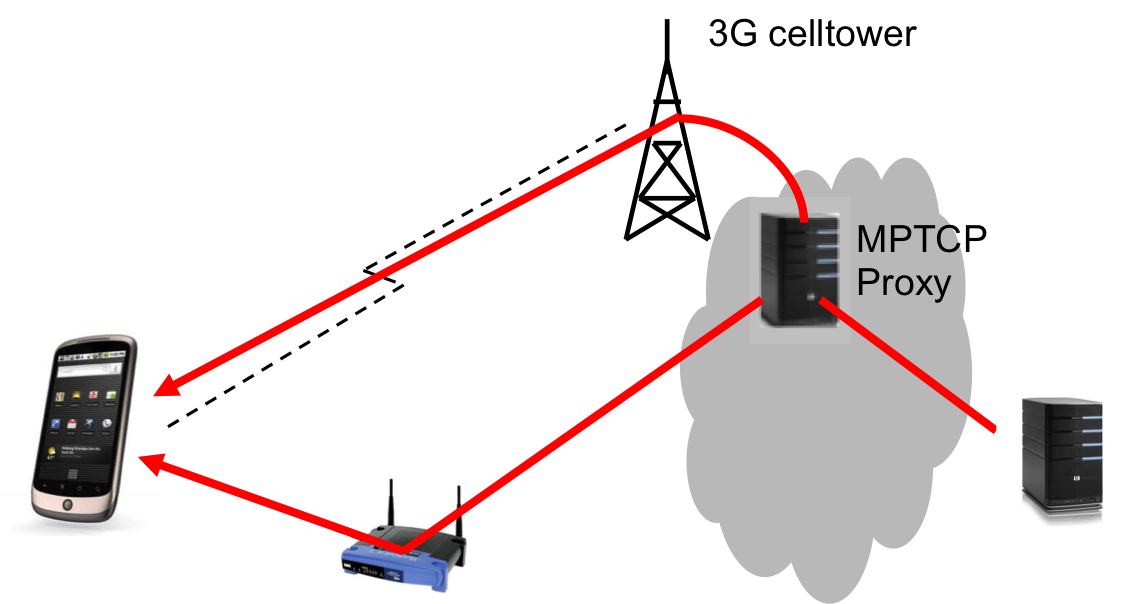
\includegraphics[scale=0.7]{figures/45g_proxy.png}
	\caption{Comunicația prin proxy}
    	\label{fig:proxy}
\end{figure}

Metricile folosite au fost round-trip time (RTT) și throughput. S-au folosit scripturi Python și utilitare open-source pentru măsurarea valorilor acestor metrici în scenariile considerate.

Tabelul \ref{tab:rtt} prezintă valorile RTT-ului în cele 3 scenarii. Pentru acest experiment s-a implementat un script Python care trimite date la un server si masoara timpul pana la primirea raspunsului. S-au trimis date de 1000 de ori si s-au calculat statistici pe baza timpului obținut la fiecare iterație (minim, maxim, media, mediana, deviația standard).

Se poate observa că nu există o diferență notabilă între comunicația directă cu TCP și cea cu MPTCP din punct de vedere al RTT-ului. Folosirea unui proxy introduce o latență de aproximativ 3ms, care este o valoare acceptabilă deoarece nu afectează calitatea experienței utilizatorului.

\begin{table}[h]
\centering
\caption{RTT}
\label{tab:rtt}
\begin{tabular}{l | c c}
\hline
& Interval RTT (ms)  & RTT median (ms) \\
\hline
Telefon --(TCP) --$>$ Server  & 3-9 &  7.08  \\
Telefon --(MPTCP) --$>$ Server  & 3-8  & 7.29 \\
Telefon --(MPTCP)--$>$ Proxy --(TCP)--$>$ Server & 5-11  & 10.28 \\
\hline
\end{tabular}
\end{table}

Tabelul \ref{tab:throughput} prezintă valorile throughput-ului în următoarele scenarii: 1) comunicația directă între o stație desktop (prin Ethernet) și server, fara proxy, 2) comunicația directă între o stație desktop (prin WiFi) și server, fara proxy, 2) comunicația directă între mobil (prin WiFi) și server, fără proxy, 3) comunicația între mobil (prin WiFi) și server, prin proxy.

\begin{table}[h]
\centering
\caption{Throughput}
\label{tab:throughput}
\begin{tabular}{l | p{1.5cm} p{1.5cm} p{1.5cm} p{1.5cm}}
\hline
& Uplink (average) & Uplink (max) & Downlink (average) & Downlink (max) \\
\hline
Stație (eth) --$>$ Server & 933 & 945 & 501 & 611 \\
Stație (wifi) --$>$ Server & 582  & 600  & 501  & 566  \\
Telefon (wifi) --$>$ Server & 497 & 516 & 533 & 562 \\
Telefon (wifi) --$>$ Proxy --$>$ Server & 233 & 287 & 317 & 413 \\
\hline
\end{tabular}
\end{table}

În urma rezultatelor obținute, se poate observa că folosirea interfeței WiFi în loc de Ethernet, reduce considerabil throughput-ul traficului de la client la server (uplink). De asemenea, observăm că  folosirea unui proxy reduce throughput-ul atât la uplink cât și la downlink.

\section{Planul de colectare și corelare al datelor}

Următorul pas este efectuarea unui experiment în care un număr de utilizatori vor folosi în mod normal telefoane, timp de 30 de zile, cu următoarele componente software:
\begin{itemize}
	\item Protocolul MPTCP activat
	\item Aplicația ConnectivityMonitor gestionează conexiunile de WiFi și LTE și configurează tabelele de rutare MPTCP
	\item Aplicația ProxyDroid trimite tot traficul către un sistem proxy ce rulează SS5 și are MTPCP activat 
\end{itemize}

Aplicația ConnectivityMonitor va colecta periodic date legate de starea conexiunilor WiFi și LTE. Tabelul \ref{tab:date} include tipurile de date care vor fi colectate în cadrul acestui experiment.

\begin{table}[h]
\centering
\caption{Tipuri de date colectate}
\label{tab:date}
\begin{tabular}{c | c}
\hline
Interfata & Tip de date  \\
\hline
WiFi & Evenimente de conectare \\
 & Evenimente de deconectare \\
 & Număr de bytes primiți \\
 & Număr de bytes trimiși \\
 & RSSI \\
 & RTT \\
 & MCS \\
 & Frecvența \\
\hline
LTE & Evenimente de conectare \\
 & Evenimente de deconectare \\
 & Număr de bytes primiți \\
 & Număr de bytes trimiși \\
 & RSSI \\
 & CID \\
 & TAC \\
\hline
- & Nivelul bateriei \\
\hline
\end{tabular}
\end{table}

Baza de date, ce va contine valorile colectate, de pe fiecare telefon va fi trimisă periodic în Cloud, în spațiul de stocare Firebase. Datele vor fi extrase și procesate de către o componentă software separată.

Analiza datelor colectate va consta în corelarea dintre evenimentele de conectare/deconectare a interfețelor WiFi/LTE, a calității acestor conexiuni și a traficului realizat de către utilizator. Rezultatele vor indica beneficiile practice aduse de protocolul MPTCP.





\chapter{Studiu conectare MPTCP în rețeaua ORO}
\label{sec:oro_arch}

\section{Caracteristicile rețelei 3G/4G ORO}

Reţeaua ORO, prezentată în figura \ref{fig:oro_network}, oferă atât
servicii de date mobile folosind rețeaua celulară, cât şi servicii de
conectare la internet folosind reţele WiFi.  In cazul reţelei 3G/4G,
accesul se face prin echipamentele NodeB, RNC, EPG pentru sesiunile
3G, respectiv eNodeB, MME, EPG pentru sesiunile 4G, iar tot traficul
este filtrat prin echipamentele de tip Firewall, de unde se face
accesul către internet.  Orange Romania oferă si rețele Wi-Fi pentru
accesul la internet, folosindu-se de echipamente de tip Access Point,
iar traficul este agregat central in rețea in WLAN GW.  Clienții
folosesc un APN a primi acces la internet, iar clienții comerciali
folosesc APN-ul net. Pentru aceștia, opțiunile extra din protocolul
TCP precum MPTCP sunt tăiate de către Firewall-uri, așadar pentru
implementarea acestui serviciu de tip 4.5G sunt necesare configurarea
unui APN dedicat si configurarea si realizarea unei configurații
speciale in rețea pentru plasarea Proxy-ului MPTCP.

\begin{figure}[h]
	\centering
	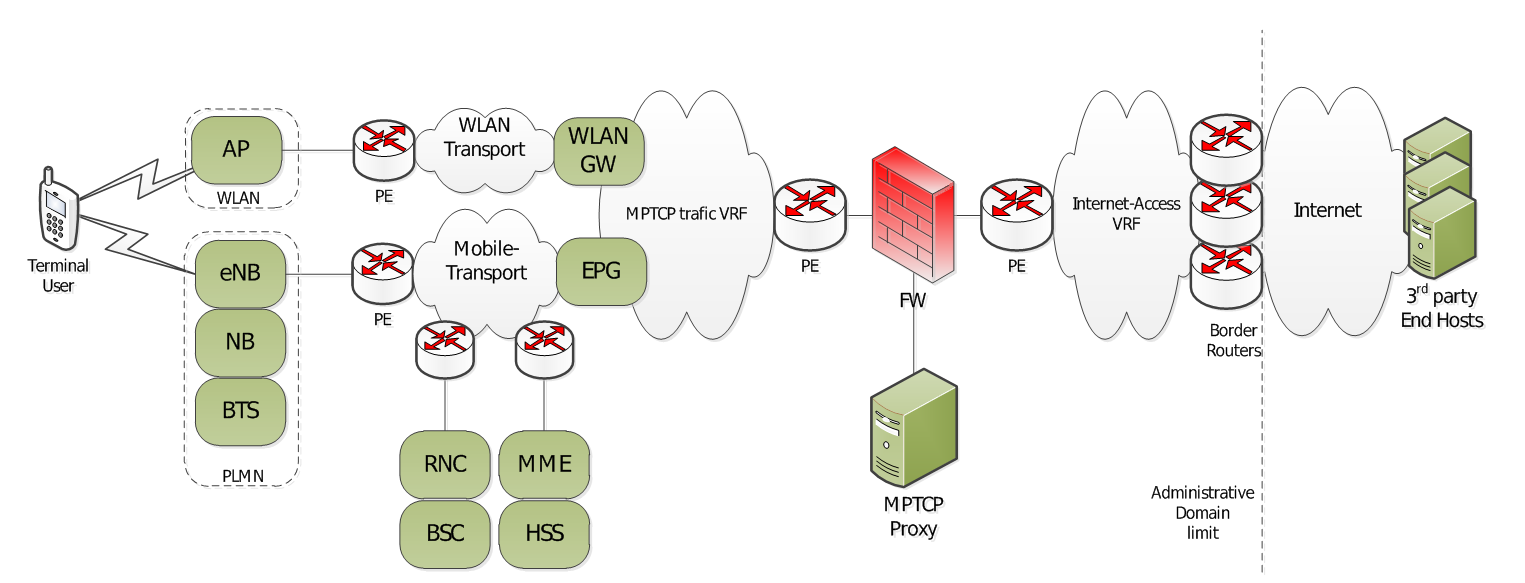
\includegraphics[scale=0.3]{figures/oro/oro_network.png}
	\caption{Structura generală a rețelei de test}
    	\label{fig:oro_network}
\end{figure}


\section{Plasarea proxy-ului MPTCP în rețeaua SGi-LAN}

\begin{figure}[h]
	\centering
	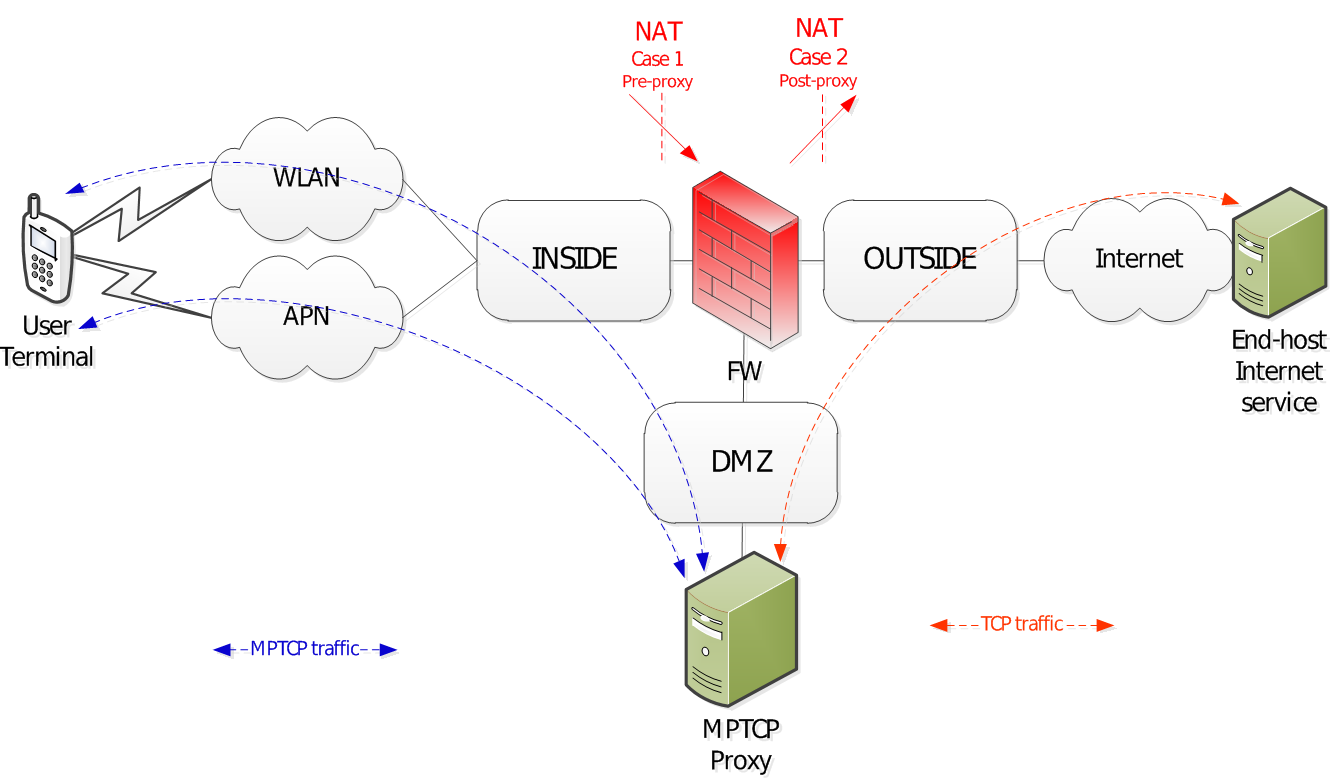
\includegraphics[scale=0.3]{figures/oro/oro_mptcp.png}
	\caption{Plasarea proxy-ului de MPTCP în spatele unui firewall cu trei zone}
    	\label{fig:oro_mptcp}
\end{figure}

Serviciul MPTCP va fi testat utilizând un APN dedicat, prin
infrastructura de date mobile și un SSID dedicat, prin intermediul
infrastructurii WLAN. Atât APN-ul, cât și SSID-ul vor folosi adresare
IP privată pentru serviciul de acces la Internet al utilizatorilor
Conectivitatea la Internet va fi asigurată folosind funcția CG-NAT44
pe un Firewall a serviciului, iar expunerea serviciilor de acces la
Internet prin intermediul unui echipament Firewall este necesară
pentru a evita intrarea pe Internet a traficului nesolicitat de la
terminalele utilizatorilor; acest trafic poate afecta autonomia
bateriilor terminalelor mobile, precum și consumul planului de date
privind abonamentele.  Se va implementa următorul design de Firewall
cu trei zone prezentat în figura \ref{fig:oro_mptcp}:
\begin{itemize}
 \item Zona FW Inside - zona APN și WLAN
 \item Zona FW DMZ -zona MPTCP Proxy
 \item Zona FW Outside- zona de internet
\end{itemize}
 
Setări pentru politica de protecție Firewall:
\begin{itemize}
 \item 	permite trafic: \\
o	Inside $\rightarrow$ DMZ\\
o	Inside  $\rightarrow$  Outside\\
o	DMZ  $\rightarrow$  Outside
\item blocarea traficului:\\
o	Outside   $\rightarrow$  Inside\\
o	Outside  $\rightarrow$  DMZ
\end{itemize}


\section{Opțiuni de instalare a funcției NAT în funcție de poziția proxy-ului de MPTCP }

Funcția de NAT va face translatarea adreselor IP private in adrese IP
publice.  Nu se va efectua traducerea adreselor pentru adresa IP de
destinație către Proxy sau Internet.  Din perspectiva dispozitivului
NAT există două opțiuni de instalare a funcției NAT:
 \\

\begin{figure}[h]
	\centering
	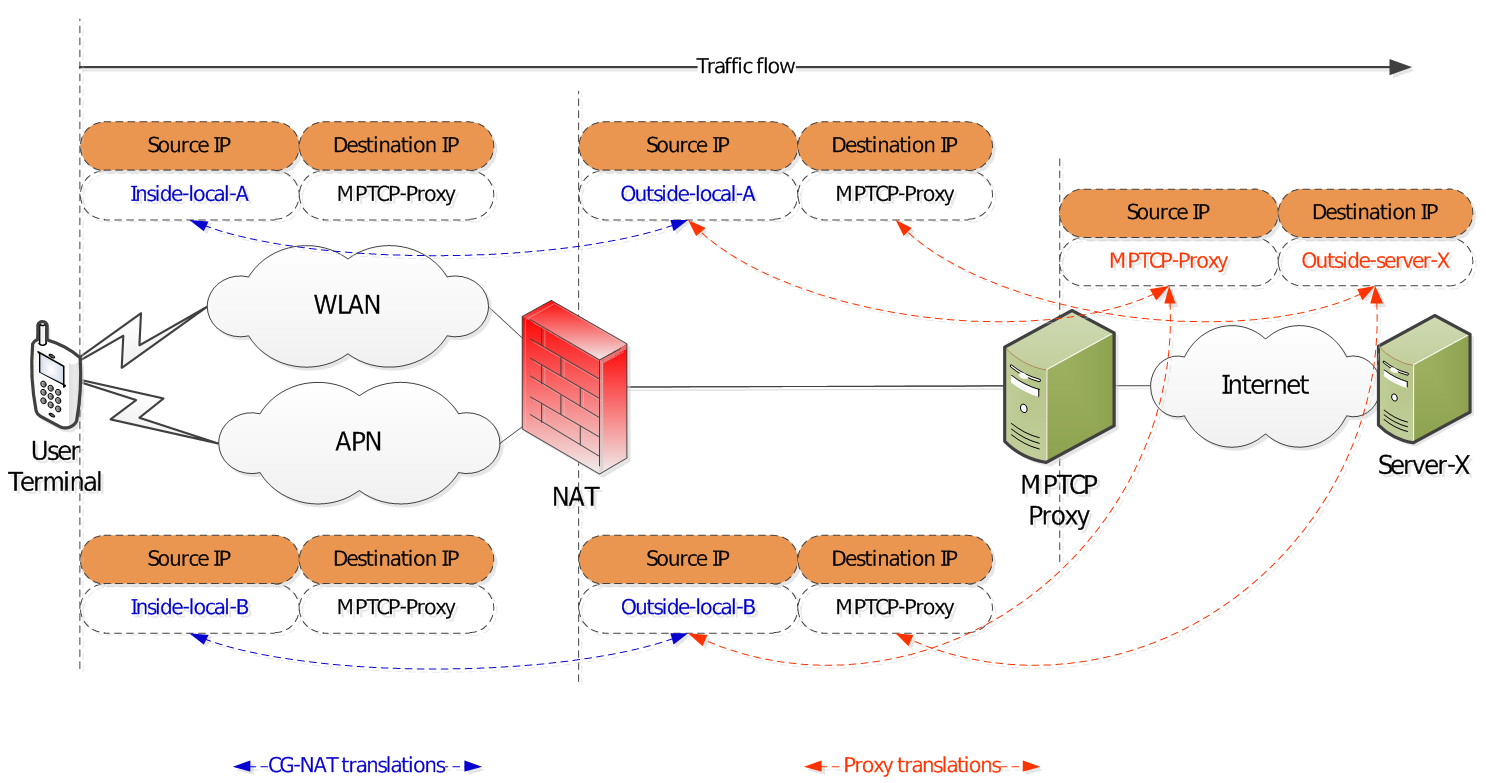
\includegraphics[scale=0.3]{figures/oro/oro_mptcp_nat.png}
	\caption{Pre-proxy NAT}
    	\label{fig:oro_mptcp_nat}
\end{figure}



{\em Cazul 1}: (figura \ref{fig:oro_mptcp_nat}) Pre-Proxy NAT – funcția NAT este plasata intre terminal si MPTCP Proxy.
\begin{itemize}
 \item	Proxy-ul trebuie să fie configurat cu o adresă IP publică sau cu un pool pentru a avea conectivitate directă la Internet.
\item Funcția NAT trebuie să fie dimensionat pentru dublul sesiunilor TCP.
\item Impactul NAT asupra funcției Proxy trebuie să fie considerat pentru o funcționare adecvată a Proxy-ului
\end{itemize}
 
  
{\em Cazul 2}: figura (\ref{fig:oro_mptcp_nat2}) Post-Proxy NAT - funcția NAT este plasata intre MPTCP Proxy si internet
\begin{itemize}
 \item	Proxy-ul poate folosi si adrese private.
\item	Există un avantaj față de cazul 1, deoarece numărul de fluxuri NAT este mai mic după Proxy, comparativ cu cazul anterior, din cauza lipsei fluxurilor MPTCP. De asemenea, protocolul MPTCP poate fi configurat cu o adresă IP publică, pentru a elimina complet necesitatea NAT pentru Proxy-ul MPTCP.
\item	Funcția NAT va rămâne în continuare pentru fluxurile de traficnon-TCP ale utilizatorilor.
 \end{itemize}
 
\begin{figure}[h]
	\centering
	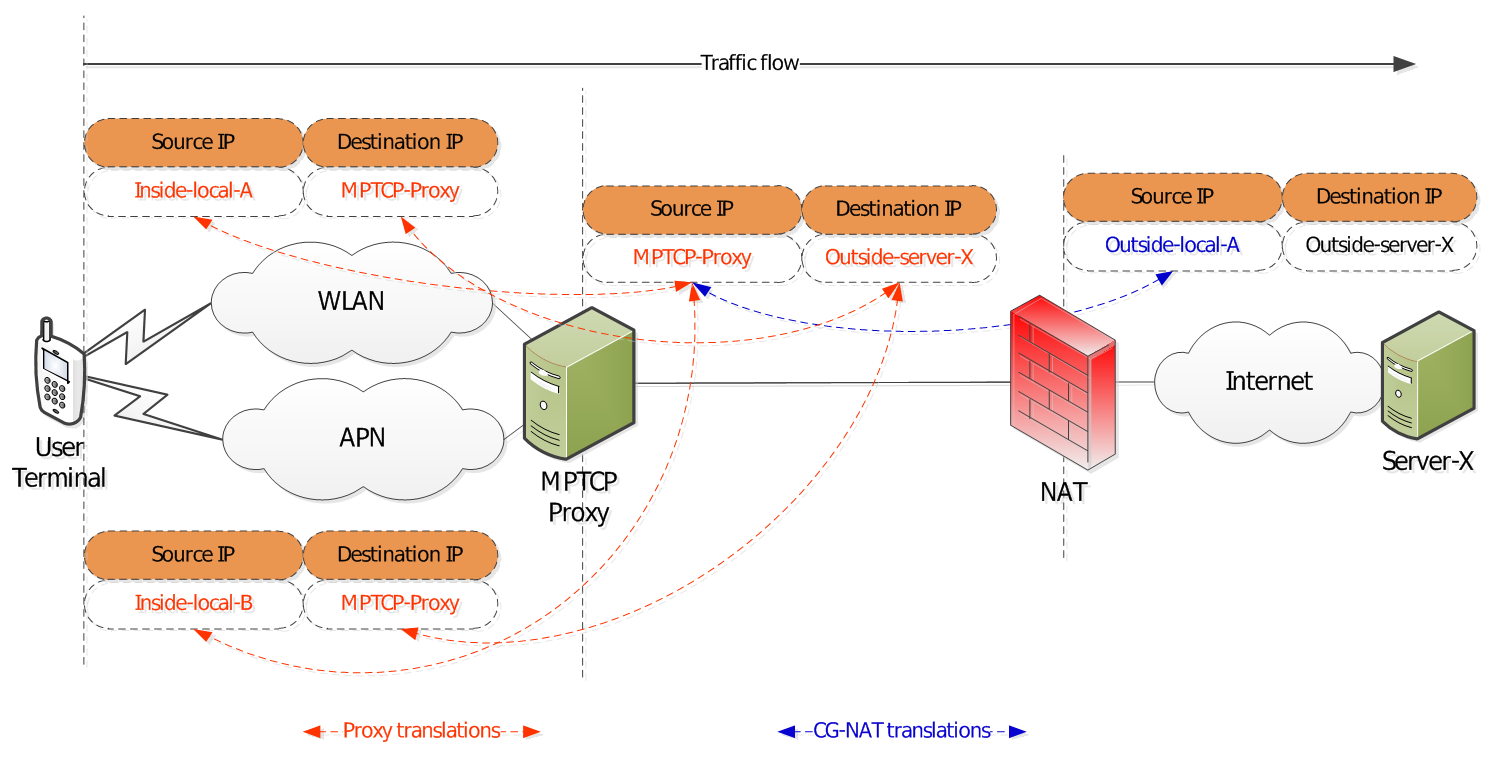
\includegraphics[scale=0.3]{figures/oro/oro_mptcp_nat2.png}
	\caption{Post-proxy NAT}
    	\label{fig:oro_mptcp_nat2}
\end{figure}




 

%%%%%%%%%%%%%%%%%%%%%%%%%%%%%%%%%%%%%%%%%%%%%%%%%%%%%%%%%%%%%%%%%%%%%-
%% INTRODUCERE - CHAPTER 1
%%%%%%%%%%%%%%%%%%%%%%%%%%%%%%%%%%%%%%%%%%%%%%%%%%%%%%%%%%%%%%%%%%%%%-

% \input{arch-basics}

%\input{faza}
%%%%%%%%%%%%%%%%%%%%%%%%%%%%%%%%%%%%%%%%%%%%%%%%%%%%%%%%%%%%%%%%%%%%%-
%% ARHITECTURA - CHAPTER 2
%%%%%%%%%%%%%%%%%%%%%%%%%%%%%%%%%%%%%%%%%%%%%%%%%%%%%%%%%%%%%%%%%%%%%-
%\input{arhitectura}


%%%%%%%%%%%%%%%%%%%%%%%%%%%%%%%%%%%%%%%%%%%%%%%%%%%%%%%%%%%%%%%%%%%%%-
%% COMPONENTE - CHAPTER 3
%%%%%%%%%%%%%%%%%%%%%%%%%%%%%%%%%%%%%%%%%%%%%%%%%%%%%%%%%%%%%%%%%%%%%-

% \chapter*{SECTIUNEA I: Stabilirea Cerintelor si Modelului Arhitectural}
% 
% \addcontentsline{toc}{chapter}{SECTIUNEA I: Stabilirea Cerintelor si Modelului Arhitectural}
% 
% \input{middlebox_study}
% 
% \input{componente}
% 
% 
% \chapter*{SECTIUNEA II: Proiectarea Platformei si Protocoalelor}
% \addcontentsline{toc}{chapter}{SECTIUNEA II: Proiectarea Platformei si Protocoalelor}
% \input{platforma}


%%%%%%%%%%%%%%%%%%%%%%%%%%%%%%%%%%%%%%%%%%%%%%%%%%%%%%%%%%%%%%%%%%%%%-
%% Aplicatii - CHAPTER 5
%%%%%%%%%%%%%%%%%%%%%%%%%%%%%%%%%%%%%%%%%%%%%%%%%%%%%%%%%%%%%%%%%%%%%-
% \input{aplicatii}

%%%%%%%%%%%%%%%%%%%%%%%%%%%%%%%%%%%%%%%%%%%%%%%%%%%%%%%%%%%%%%%%%%%%%-
%% Concluzii - CHAPTER 6
%%%%%%%%%%%%%%%%%%%%%%%%%%%%%%%%%%%%%%%%%%%%%%%%%%%%%%%%%%%%%%%%%%%%%-
% \chapter{Concluzii}
% \input{concluzii}
% 
% \chapter*{SECTIUNEA III: Stabilirea Planului de Diseminare}
% \input{dissemination}
% 
% \addcontentsline{toc}{chapter}{SECTIUNEA III: Stabilirea Planului de Diseminare}


%%%%%%%%%%%%%%%%%%%%%%%%%%%%%%%%%%%%%%%%%%%%%%%%%%%%%%%%%%%%%%%%%%%%%-
%% BIBLIOGRAPHY
%%%%%%%%%%%%%%%%%%%%%%%%%%%%%%%%%%%%%%%%%%%%%%%%%%%%%%%%%%%%%%%%%%%%%-
\addcontentsline{toc}{chapter}{Bibliografie}
\renewcommand{\bibname}{Bibliografie}

\addcontentsline{toc}{chapter}{References}
%\bibliographystyle{ieeetr}
\bibliographystyle{plain}
%\bibliographystyle{abbrv}
%\bibliographystyle{phjcp}
%%\bibliographystyle{apalike}
\bibliography{references}
% \bibliography{chapters/symnet/biblio}
%%%%%%%%%%%%%%%%%%%%%%%%%%%%%%%%%%%%%%%%%%%%%%%%%%%%%%%%%%%%%%%%%%%%%%
%%% content.tex ends here
